\chapter{METODOLOGI PENELITIAN}
\section{Tempat dan Jadwal Kegiatan Penelitian}
Dalam melaksanakan sebuah penelitian, perencanaan waktu merupakan komponen kritis yang memastikan alur penelitian dapat berjalan dengan terstruktur dan sistematis. Gambar \ref{fig:jadwal-penelitian} menyajikan jadwal penelitian yang telah dirancang untuk penelitian ini. Jadwal tersebut mencakup rentang waktu mulai dari September 2023 hingga April 2024 dan menguraikan berbagai kegiatan yang akan dilakukan selama periode tersebut. Selanjutnya, penelitian ini akan dilaksanakan di Laboratorium Komputer, Institut Teknologi Sumatera.

\begin{figure}[h!]
    \centering
    \includegraphics[width=1\textwidth]{figures/ch03/Timeline-2.png}
    \caption{Jadwal Penelitian}
    \label{fig:jadwal-penelitian}
\end{figure}


\section{Alur Penelitian}
Adapun diagram alir penelitian ini ditunjukkan pada Gambar \ref{fig:diagram alir} terdapat enam tahapan. Langkah awal yang dilakukan pada penelitian ini adalah melakukan identifikasi masalah, yaitu proses mencari, menghimpun, serta menemukan permasalahan yang nantinya akan diselesaikan. Setelah melakukan identifikasi masalah, langkah selanjutnya adalah studi literatur. Studi literatur adalah tahapan untuk mencari solusi dari permasalahan yang sebelumnya sudah kita definisikan. Pencarian solusi ini dapat melalui membaca referensi ilmiah terdahulu, baik melalui jurnal, buku, dokumentasi resmi, tesis, dan lain-lain. Tahapan ini akan memberikan pemahaman mendasar mengenai permasalahan yang sudah didapatkan sebelumnya. 

\begin{figure}[h!]
    \centering
    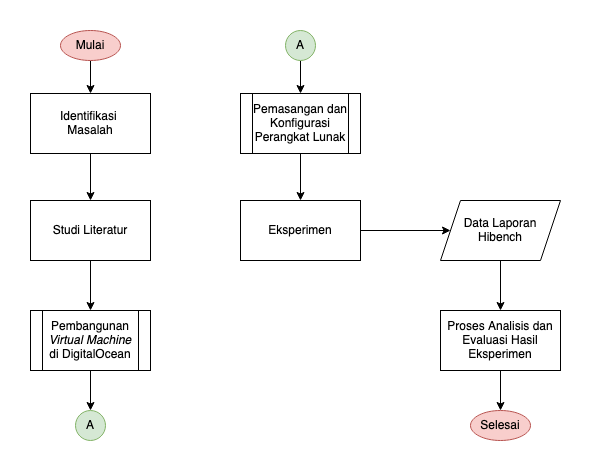
\includegraphics[width=0.9\textwidth]{figures/ch03/Diagram Tugas Akhir.png}
    \caption{Diagram Alir Penelitian}
    \label{fig:diagram alir}
\end{figure}

Kemudian, penelitian ini akan dilanjutkan pada tahap membangun \textit{virtual machine} di DigitalOcean. DigitalOcean adalah perusahaan penyedia layanan awan \textit{Infrastructure as a Service} (IaaS) yang memberikan banyak pilihan kepada pengguna untuk menggunakan berbagai jenis layanan sesuai dengan kebutuhan, salah satunya yaitu \textit{virtual machine}. \textit{Virtual Machine} tersebut dapat dihentikan atau dihapus kapanpun saat tidak lagi diperlukan. Ketika infrastruktur sudah siap digunakan, penelitian dilanjutkan ke tahap pemasangan perangkat lunak, seperti Hadoop, Spark, dan HiBench. Selanjutnya dilakukan eksperimen pada beban kerja \textit{Micro Benchmarks}. Akhirnya, hasil dari eksperimen akan digunakan untuk proses analisis dan evaluasi.

\section{Penjabaran Langkah Penelitian}
Adapun untuk lebih memperjelas lagi dari setiap langkah yang ada pada Gambar \ref{fig:diagram alir}, dijabarkan secara rinci tahapan-tahapan yang dilakukan pada penelitian ini.

\subsection{Identifikasi Masalah dan Studi Literatur}
Langkah awal penelitian ini adalah identifikasi masalah dan studi literatur. Identifikasi masalah dapat dipahami sebagai tahapan mendefinisikan masalah sehingga masalah tersebut dapat terukur dan jelas untuk dijadikan landasan dalam latar belakang penelitian. Setelah masalah berhasil diidentifikasi, langkah selanjutnya adalah studi literatur yang mana dalam proses ini dilakukan pengumpulan berbagai macam informasi, referensi, dan konsep dasar yang menjadi landasan dasar dari penelitian. Langkah ini dapat dilakukan melalui membaca artikel ilmiah pendukung, buku-buku yang ditulis oleh para ahli, dan jika berkaitan dengan pemrograman dapat melihat dari dokumentasi resmi. Pada tahap ini juga dilakukan analisis terhadap penelitian terdahulu dan dibandingkan dengan identifikasi masalah yang didapatkan untuk membuka celah penelitian baru sehingga penelitian ini dapat bermanfaat. 

\subsection{Membangun \textit{Virtual Machine} di DigitalOcean}
Konfigurasi perangkat keras merupakan aspek penting dalam mengevaluasi kinerja aplikasi \textit{big data} berbasis Hadoop dan Spark. DigitalOcean, sebagai penyedia layanan infrastruktur sebagai layanan (IaaS), memberikan pengguna kebebasan penuh untuk membuat, mengonfigurasi, dan mengelola berbagai infrastruktur yang telah disediakan. Dalam konteks penelitian ini, diperlukan penggunaan mesin virtual, yang dalam DigitalOcean dikenal sebagai "Droplets," yang memungkinkan untuk menyesuaikan berbagai aspek seperti sistem operasi, kapasitas penyimpanan, jumlah prosesor, dan parameter lainnya sesuai dengan kebutuhan spesifik penelitian.

\begin{table}[h!]
	\centering
	\caption{Konfigurasi Perangkat Keras}
	\begin{tabular}{|ll|}
		\hline
		\multicolumn{1}{|c|}{\textbf{Nama Parameter}}    & \multicolumn{1}{c|}{\textbf{Nilai Parameter}} \\ \hline
		\multicolumn{1}{|l|}{\textbf{Lokasi Pusat Data}} & Singapore - Datacenter 1 - SGP1               \\ \hline
		\multicolumn{1}{|l|}{\textbf{Sistem Operasi}}    & Ubuntu 20.04 (LTS) x64                        \\ \hline
		\multicolumn{1}{|l|}{\textbf{Jenis Droplet}}     & Basic                                         \\ \hline
		\multicolumn{1}{|l|}{\textbf{Prosesor}}          & Premium AMD - 4 Core                          \\ \hline
		\multicolumn{1}{|l|}{\textbf{Memori}}            & 8 GB                                          \\ \hline
		\multicolumn{1}{|l|}{\textbf{Penyimpanan}}       & 160 GB NVMe SSD                               \\ \hline
	\end{tabular}
	\label{table:conf-hardware}
\end{table}

Penelitian ini mengadopsi mode \textit{pseudo-distributed} yang memungkinkan penggunaan hanya satu \textit{virtual machine} dalam konfigurasi \textit{single node}. Walaupun hanya menggunakan satu \textit{virtual machine}, mode \textit{pseudo-distributed} memungkinkan setiap proses dalam klaster beroperasi secara independen, menciptakan lingkungan di mana semua proses berjalan mandiri satu sama lain. Hal ini memungkinkan untuk lebih berfokus pada pengumpulan data dan analisis, tanpa perlu melakukan konfigurasi yang rumit terkait dengan pengaturan klaster. Spesifikasi perangkat keras yang digunakan untuk \textit{virtual machine} dalam mode \textit{pseudo-distributed} sesuai pada Tabel \ref{table:conf-hardware}. Penjelasan lengkap tentang pembuatan \textit{virtual machine} (VM) pada \textit{platform} DigitalOcean dan cara mengakses VM tersebut disajikan pada Lampiran \ref{appendix:A}.

\subsection{Pemasangan dan Konfigurasi Perangkat Lunak}
Pemasangan dan konfigurasi perangkat lunak merupakan hal yang krusial dalam penelitian ini. Perangkat lunak yang diperlukan ditunjukkan pada Tabel \ref{table:software-needs}.

\begin{table}[h]
	\centering
	\caption{Perangkat Lunak yang Dibutuhkan}
		\begin{tabular}{|c|p{9cm}|}
		\hline
			\textbf{Perangkat Lunak} & \multicolumn{1}{c|}{\textbf{Deskripsi}}                                                                                \\ \hline
			Ubuntu 20.04 LTS x64     & Sistem operasi Linux berbasis Ubuntu  \\ \hline
			Git                      & Sistem kontrol versi untuk mengelola perubahan dalam kode sumber perangkat lunak                                       \\ \hline
			Maven                    & Perangkat lunak manajemen proyek Java                            \\ \hline
			Java 8                   & \multirow{3}{*}{Bahasa pemrograman dasar}                                 \\ \cline{1-1}
			Python 3.7               &                                                                                                                        \\ \cline{1-1}
			Scala 2.x               &                                                                                                                        \\ \hline
			Hadoop                & Perangkat lunak pengolahan data terdistribusi untuk penyimpanan dan manajemen data besar                               \\ \hline
			Spark               & Kerangka kerja pemrosesan data terdistribusi yang berjalan di atas Hadoop                                              \\ \hline
			Hibench   & Alat yang digunakan untuk mengukur kinerja Hadoop dan Spark                                                            \\ \hline
		\end{tabular}
	\label{table:software-needs}
\end{table}

Alur kerja instalasi perangkat lunak dalam penelitian ini dapat dilihat pada Gambar \ref{fig:alurkerja-soft}. Pada gambar, terdapat tiga bagian utama, yaitu \textit{prerequisites} (perangkat lunak prasyarat) ditandai dengan warna biru, alat penyimpanan dan pemrosesan \textit{Big Data} ditandai dengan warna oren, dan alat untuk mengukur kinerja \textit{big data} ditandai dengan warna hijau. Semua perangkat lunak dijalankan pada sistem operasi Ubuntu 20.04 LTS x64.

\begin{figure}[h]
    \centering
    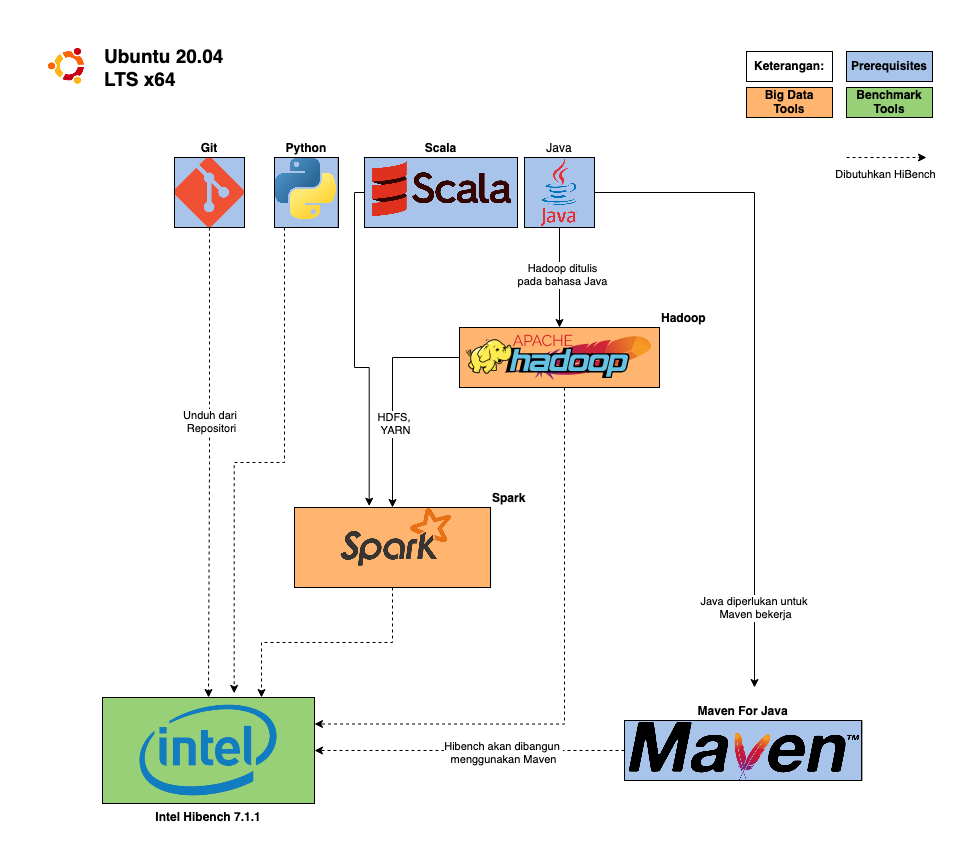
\includegraphics[width=1\textwidth]{figures/ch03/alurkerja-soft.png}
    \caption{Alur Instalasi Perangkat Lunak}
    \label{fig:alurkerja-soft}
\end{figure}

\subsubsection{Instalasi Perangkat Lunak Prasyarat}
Ada beberapa perangkat lunak yang perlu diimplementasikan sebelum memasang Hadoop, Spark, Hive, dan HiBench, yaitu:
\begin{enumerate}
	\item Ubuntu 20.04 LTS x64
	\item Git
	\item Java 8 dan Maven
	\item Python 3.7
	\item Scala 2.x
\end{enumerate}

Pemasangan dan konfigurasi perangkat lunak pada tahapan ini tidak membutuhkan urutan. Akan tetapi, pada penelitian ini dibuatkan alur untuk pemasangan dan konfigurasi perangkat lunak prasyarat seperti pada Gambar \ref{fig:prasyarat-flow}. Penjelasan lengkap mengenai tata cara instalasi dan konfigurasi perangkat lunak prasyarat ini disajikan pada Lampiran \ref{appendix:B}. 

\begin{figure}[h!]
    \centering
    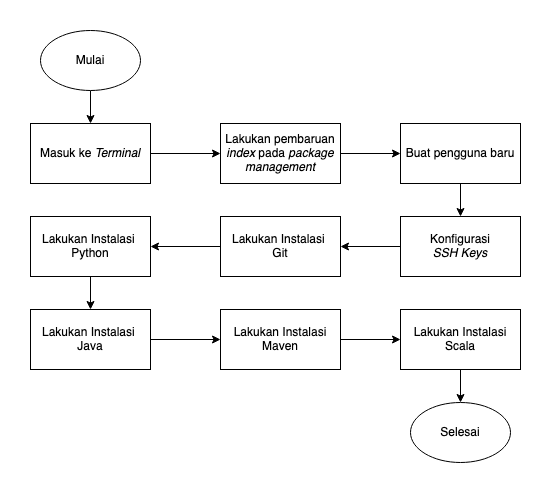
\includegraphics[width=0.75\textwidth]{figures/ch03/prasayarat-flow.png}
    \caption{Alur Instalasi Perangkat Lunak Prasyarat}
    \label{fig:prasyarat-flow}
\end{figure}


\subsubsection{Instalasi dan Konfigurasi Hadoop}
Hadoop adalah perangkat lunak \textit{open source} yang efektif dalam menyimpan dan memproses data dalam skala besar. Daripada menggunakan satu komputer besar untuk menyimpan dan memproses data, Hadoop memungkinkan pengklasteran beberapa komputer untuk menganalisis set data besar secara paralel dengan lebih cepat. Ada beberapa perangkat lunak prasyarat yang perlu dipasang sebelum menggunakan Hadoop. Setelah perangkat lunak prasyarat berhasil dipasang, Hadoop juga dapat dipasang mengikuti panduan lengkap pada Lampiran \ref{appendix:C}. 
Secara umum, alur yang harus dilakukan meliputi pengunduhan berkas Hadoop. Selanjutnya akan dilakukan pengubahan kepemilikan berkas ke \textit{user hdfsuser}. Karena Hadoop tidak mendukung IPv6, maka fitur ini perlu dimatikan juga. Alur pemasangan dan konfigurasi Hadoop lebih jelas sesuai dengan Gambar \ref{fig:hadoop-flow}.

\begin{figure}[h!]
    \centering
    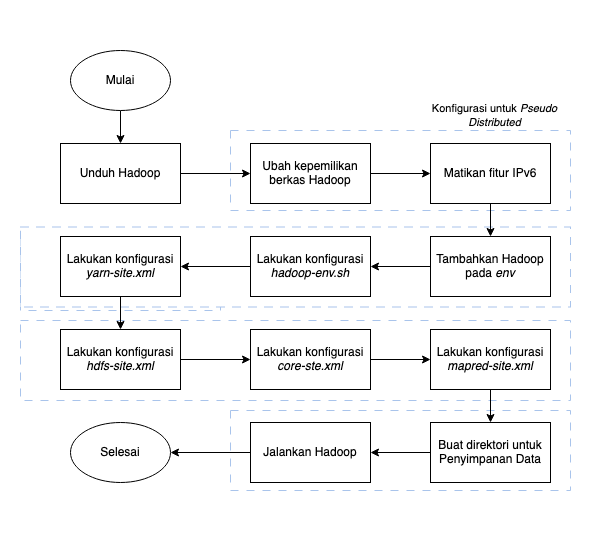
\includegraphics[width=0.6\textwidth]{figures/ch03/hadoop-flow.png}
    \caption{Alur Instalasi dan Konfigurasi Hadoop}
    \label{fig:hadoop-flow}
\end{figure}

\subsubsection{Instalasi dan Konfigurasi Spark}
Apache Spark adalah sebuah kerangka kerja pengolahan data terdistribusi yang sangat cepat dan efisien. Spark dan Hadoop memiliki hubungan yang erat. Spark dapat berjalan di atas \textit{Hadoop Distributed File System} (HDFS) dan dapat menggunakan Hadoop YARN sebagai manajer sumber daya. Oleh karena itu, instalasi Spark membutuhkan Hadoop sudah terpasang lebih dahulu. Alur pemasangan dan konfigurasi spark terlihat seperti pada Gambar \ref{fig:spark-flow}. Apabila Hadoop sudah berhasil terpasang, langkah selanjutnya adalah memasang Spark seperti pada Lampiran \ref{appendix:D}.

\begin{figure}[h]
    \centering
    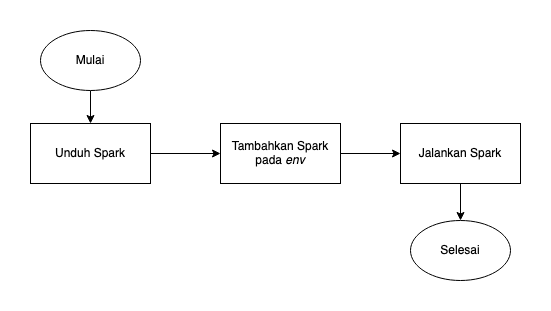
\includegraphics[width=0.7\textwidth]{figures/ch03/spark-flow.png}
    \caption{Alur Instalasi dan Konfigurasi Spark}
    \label{fig:spark-flow}
\end{figure}

\subsubsection{Instalasi dan Konfigurasi HiBench}
Sebelum melakukan eksperimen, diperlukan suatu perangkat lunak pengukuran kinerja sistem \textit{Big Data}, yaitu HiBench. HiBench tidak dapat digunakan secara langsung ketika sudah berhasil diunduh, melainkan harus dilakukan pembangunan beberapa modul yang dibutuhkan dengan Maven dan konfigurasi beberapa parameter. Secara umum, alur instalasi dan konfigurasi HiBench sesuai dengan Gambar \ref{fig:hibench-flow}. Berkas HiBench diunduh dari repositori, dilanjutkan dengan pembangunan beberapa modul yang nantinya dibutuhkan. Selanjutnya, dilakukan konfigurasi beberapa berkas seperti \textit{hibench.conf, hadoop.conf, dan spark.conf}. Jika telah dilakukan konfigurasi, dapat dilanjutkan dengan menjalankan beban kerja atau eksperimen. Lebih lanjut, pemasangan dan konfigurasi HiBench dijelaskan pada Lampiran \ref{appendix:E}.

\begin{figure}[h]
    \centering
    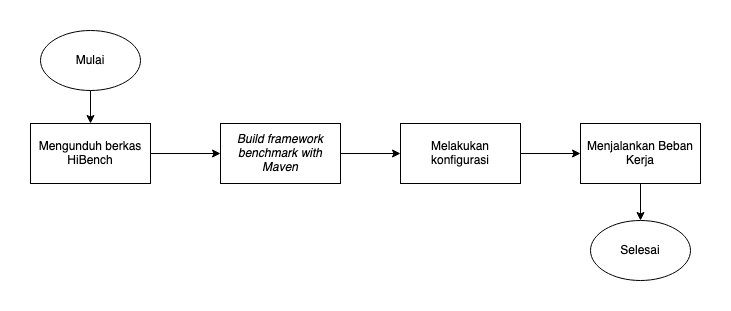
\includegraphics[width=0.9\textwidth]{figures/ch03/hibench-flow.png}
    \caption{Alur Instalasi dan Konfigurasi HiBench}
    \label{fig:hibench-flow}
\end{figure}

\subsection{Eksperimen}
Eksperimen merupakan tahapan yang dilakukan setelah perangkat keras dan perangkat lunak sudah berhasil terpasang. Pada tahapan ini, dilakukan berbagai percobaan untuk menjawab pertanyaan pada masalah yang sebelumnya sudah didefinisikan. Beberapa beban kerja yang akan diuji coba pada tahapan ini dapat dilihat pada Tabel \ref{table:workload}. 

\begin{table}[h!]
\caption{Beban Kerja yang Digunakan}
\label{table:workload}
\resizebox{\textwidth}{!}{%
\begin{tabular}{|l|l|l|l|}
\hline
\multicolumn{1}{|c|}{\begin{tabular}[c]{@{}c@{}}Tipe Beban \\ Kerja\end{tabular}} & \multicolumn{1}{c|}{Nama Beban Kerja} & \multicolumn{1}{c|}{Sumber Data} & \multicolumn{1}{c|}{Perangkat Lunak} \\ \hline
\multirow{3}{*}{\begin{tabular}[c]{@{}l@{}}Micro \\ Benchmarks\end{tabular}} & Sort & RandomTextWriter & \multirow{3}{*}{Hadoop, Spark} \\ \cline{2-3}
 & WordCount & RandomTextWriter &  \\ \cline{2-3}
 & TeraSort & Hadoop TeraGen &  \\ \hline
\end{tabular}%
}
\end{table}

Pengujian dimulai dengan mengeksekusi beban kerja \textit{Micro Benchmarks}, yang terdiri dari \textit{WordCount, Sort, dan TeraSort}, pada DigitalOcean menggunakan parameter data yang divariasikan, yaitu {1GB; 5 GB; 10GB; 25 GB; dan 50 GB}. Parameter input data dapat disesuaikan pada berkas \textit{hibench.conf}. Hasil yang diukur berupa lama waktu eksekusi (\textit{execution time}) dan \textit{throughput per node}. Uji coba yang dijalankan pada HiBench dilakukan sebanyak masing-masing satu uji coba. Pengujian secara lengkap sesuai pada Tabel \ref{table:eksperimen}. Hasil dan konfigurasi dari setiap pengujian dapat diakses melalui berkas \textit{HiBench Report} yang nantinya akan diproses lebih lanjut pada tahap analisis dan evaluasi.

\begin{table}[h!]
\caption{Eksperimen yang Akan diuji Coba}
\label{table:eksperimen}
\resizebox{\textwidth}{!}{%
\begin{tabular}{|l|l|l|c|}
\hline
\multicolumn{1}{|c|}{Beban Kerja} & \multicolumn{1}{c|}{Input Data} & \multicolumn{1}{c|}{\begin{tabular}[c]{@{}c@{}}Perangkat \\ Lunak\end{tabular}} & Hasil yang Diukur \\ \hline
Sort, TeraSort, WordCount & 1 GB & Hadoop & \multirow{10}{*}{\textit{\begin{tabular}[c]{@{}c@{}}Execution time, \\ throughput per node\end{tabular}}} \\ \cline{1-3}
Sort, TeraSort, WordCount & 5 GB & Hadoop &  \\ \cline{1-3}
Sort, TeraSort, WordCount & 10 GB & Hadoop &  \\ \cline{1-3}
Sort, TeraSort, WordCount & 25 GB & Hadoop &  \\ \cline{1-3}
Sort, TeraSort, WordCount & 50 GB & Hadoop &  \\ \cline{1-3}
Sort, TeraSort, WordCount & 1 GB & Spark &  \\ \cline{1-3}
Sort, TeraSort, WordCount & 5 GB & Spark &  \\ \cline{1-3}
Sort, TeraSort, WordCount & 10 GB & Spark &  \\ \cline{1-3}
Sort, TeraSort, WordCount & 25 GB & Spark &  \\ \cline{1-3}
Sort, TeraSort, WordCount & 50 GB & Spark &  \\ \hline
\end{tabular}%
}
\end{table}

\subsection{Proses Analisis dan Evaluasi Hasil Eksperimen}
Analisis pada penelitian ini dilakukan dengan membandingkan hasil setiap eksperimen yang sebelumnya sudah dilakukan. Data yang akan dianalisis didapatkan melalui data eksperimen sebelumnya pada berkas \textit{hibench.report}. Selanjutnya, tahapan ini ditutup dengan evaluasi terhadap hasil dari analisis yang diperoleh.








